\documentclass[border=10pt]{standalone}
\usepackage[svgnames]{xcolor}
\usepackage{amsmath}
\usepackage{pgfplots}
\pgfplotsset{compat=newest}
\usepackage[sfdefault]{FiraSans}
\usepackage{FiraMono}
\renewcommand*\familydefault{\sfdefault}
\begin{document}
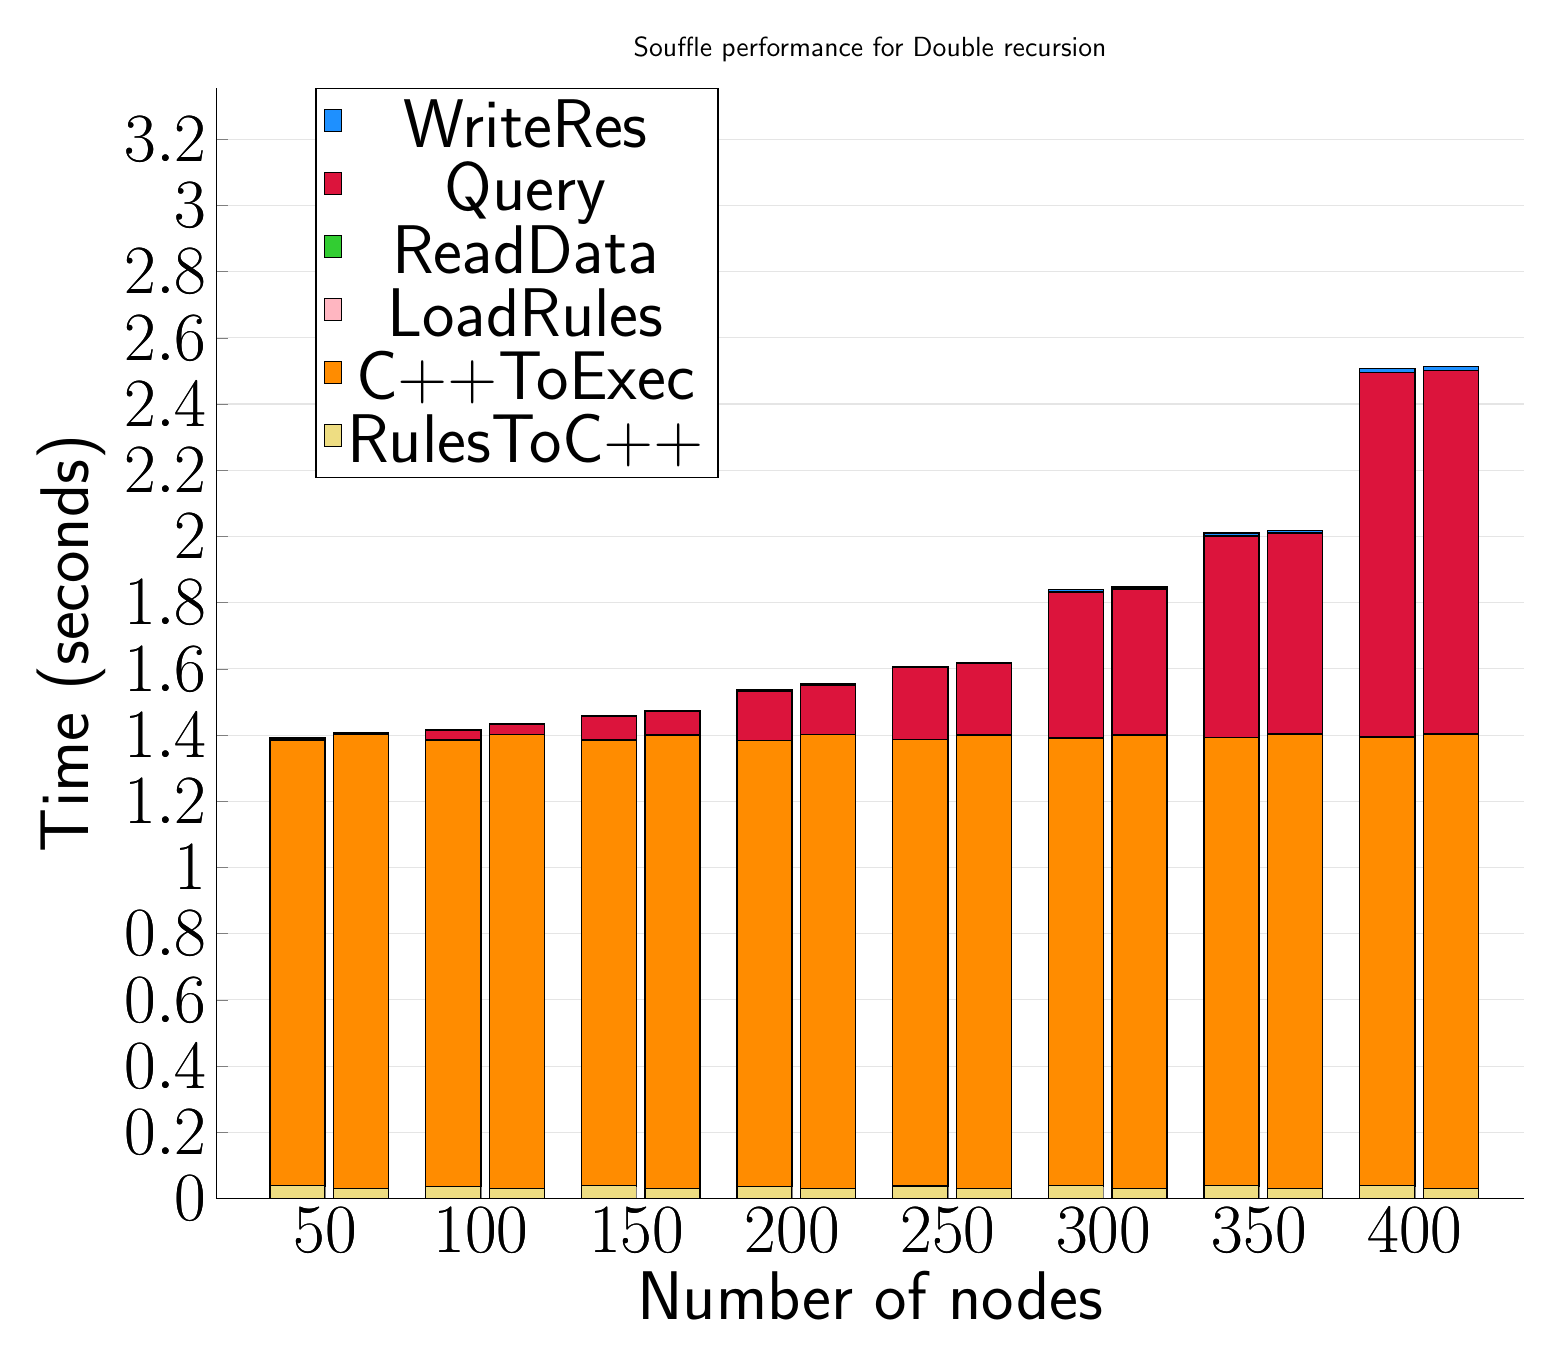
\begin{tikzpicture}
	\begin{axis}[
			ybar stacked,
			title={Souffle performance for Double recursion},
			bar shift=-10pt,
			width=1.5\textwidth,
			bar width=0.7cm,
			ymajorgrids, tick align=inside,
			major grid style={draw=gray!20},
			xtick=data,
			ymin=0, ymax=3.3549999952316285,
			axis x line*=bottom,
			axis y line*=left,
			enlarge x limits=0.1,
			legend style={
					at={(0.23, 1)},
					anchor=north,
					legend columns=1,
					font=\Huge,
				},
			ylabel={Time (seconds)},
			xlabel={Number of nodes},
			label style={font=\Huge},
			tick label style={font=\Huge},
		]
		\addlegendimage{fill=DodgerBlue, draw=black, line width=0.2pt}
		\addlegendentry{WriteRes}
		\addlegendimage{fill=Crimson, draw=black, line width=0.2pt}
		\addlegendentry{Query}
		\addlegendimage{fill=LimeGreen, draw=black, line width=0.2pt}
		\addlegendentry{ReadData}
		\addlegendimage{fill=LightPink, draw=black, line width=0.2pt}
		\addlegendentry{LoadRules}
		\addlegendimage{fill=DarkOrange, draw=black, line width=0.2pt}
		\addlegendentry{C++ToExec}
		\addlegendimage{fill=LightGoldenrod, draw=black, line width=0.2pt}
		\addlegendentry{RulesToC++}
		\addplot +[fill=LightGoldenrod, draw=black, line width=0.5pt] coordinates {
				(50, 0.03900001049041748)
				(100, 0.03599998950958252)
				(150, 0.03900001049041748)
				(200, 0.036999988555908206)
				(250, 0.037999963760375975)
				(300, 0.04000000953674317)
				(350, 0.04000000953674317)
				(400, 0.03899998664855957)
			};
		\addplot +[fill=DarkOrange, draw=black, line width=0.5pt] coordinates {
				(50, 1.3459999799728393)
				(100, 1.3480000019073486)
				(150, 1.3459999799728393)
				(200, 1.3460000276565551)
				(250, 1.347999906539917)
				(300, 1.3509999990463257)
				(350, 1.3519999980926514)
				(400, 1.3549999952316285)
			};
		\addplot +[fill=LightPink, draw=black, line width=0.5pt] coordinates {
				(50, 0.00011864170000000001)
				(100, 0.00011344580000000001)
				(150, 0.0001175291)
				(200, 0.00011187110000000001)
				(250, 0.0001139581)
				(300, 0.00011278340000000001)
				(350, 0.0001016667)
				(400, 0.00010331669999999999)
			};
		\addplot +[fill=LimeGreen, draw=black, line width=0.5pt] coordinates {
				(50, 0.0004147998)
				(100, 0.0005772041999999998)
				(150, 0.0007778126)
				(200, 0.0009679333)
				(250, 0.0010805789)
				(300, 0.001338266)
				(350, 0.0014544410000000001)
				(400, 0.0018234069999999998)
			};
		\addplot +[fill=Crimson, draw=black, line width=0.5pt] coordinates {
				(50, 0.005121016000000001)
				(100, 0.03108653)
				(150, 0.07079163000000001)
				(200, 0.1492397)
				(250, 0.21612929999999997)
				(300, 0.44018560000000007)
				(350, 0.6080009)
				(400, 1.099397)
			};
		\addplot +[fill=DodgerBlue, draw=black, line width=0.5pt] coordinates {
				(50, 0.0005344124)
				(100, 0.0011808410000000002)
				(150, 0.0018482620000000003)
				(200, 0.0032821200000000003)
				(250, 0.004211136999999999)
				(300, 0.006741201)
				(350, 0.009401922)
				(400, 0.0123846)
			};
	\end{axis}
	\begin{axis}[
			ybar stacked,
			bar shift=13pt,
			width=1.5\textwidth,
			bar width=0.7cm,
			ymajorgrids, tick align=inside,
			major grid style={draw=none},
			xtick=data,
			ymin=0, ymax=3.3549999952316285,
			axis x line*=none,
			axis y line*=none,
			enlarge x limits=0.1,
			label style={font=\Huge},
			tick label style={font=\Huge},
		]
		\addplot +[fill=LightGoldenrod, draw=black, line width=0.5pt] coordinates {
				(50, 0.030000000000000006)
				(100, 0.030000000000000006)
				(150, 0.030000000000000006)
				(200, 0.030000000000000006)
				(250, 0.030000000000000006)
				(300, 0.030000000000000006)
				(350, 0.030000000000000006)
				(400, 0.030999999999999993)
			};
		\addplot +[fill=DarkOrange, draw=black, line width=0.5pt] coordinates {
				(50, 1.3710000000000004)
				(100, 1.3720000000000003)
				(150, 1.3700000000000003)
				(200, 1.3710000000000004)
				(250, 1.3690000000000004)
				(300, 1.3700000000000003)
				(350, 1.3720000000000003)
				(400, 1.3710000000000004)
			};
		\addplot +[fill=LightPink, draw=black, line width=0.5pt] coordinates {
				(50, 0.00011770000000000001)
				(100, 0.0001126)
				(150, 0.0001167)
				(200, 0.00011100000000000001)
				(250, 0.00011310000000000001)
				(300, 0.0001121)
				(350, 0.00010089999999999999)
				(400, 0.00010250000000000001)
			};
		\addplot +[fill=LimeGreen, draw=black, line width=0.5pt] coordinates {
				(50, 0.00041410000000000004)
				(100, 0.0005765)
				(150, 0.0007771999999999999)
				(200, 0.0009673000000000001)
				(250, 0.0010798000000000001)
				(300, 0.0013373)
				(350, 0.0014536)
				(400, 0.0018224)
			};
		\addplot +[fill=Crimson, draw=black, line width=0.5pt] coordinates {
				(50, 0.0051183999999999995)
				(100, 0.0310461)
				(150, 0.070655)
				(200, 0.14891610000000002)
				(250, 0.2156725)
				(300, 0.4393192)
				(350, 0.6068296999999999)
				(400, 1.097572)
			};
		\addplot +[fill=DodgerBlue, draw=black, line width=0.5pt] coordinates {
				(50, 0.0005337)
				(100, 0.0011785)
				(150, 0.0018414)
				(200, 0.0032789)
				(250, 0.0041971)
				(300, 0.0067284)
				(350, 0.008402499999999999)
				(400, 0.012357299999999998)
			};
	\end{axis}
\end{tikzpicture}

\end{document}
